\chapter{内分泌与稳态}\label{ch:b3:endocrinology}

1921 年夏天，两名年轻人在多伦多一间闷热的实验室里结扎
了狗的胰管，等待消化组织
萎缩，研磨剩下的部分，将提取液注射到一只
因切除胰腺而患\omterm{def:b3:endocrinology:glucose}{糖尿病}的狗体内，它的血糖下降了。到了
次年一月，多伦多总医院里一名十四岁、因\omterm{def:b3:endocrinology:glucose}{糖尿病}濒死的男孩
开始接受这种提取物，几周之内他就能进食、
行走，体重也有所增加；此后他又活了十三年。这种
物质就是\omterm{def:b3:endocrinology:glucose}{胰岛素}，它是由五十一个氨基酸组成的肽，由
胰腺中占百分之一的部分分泌入血液，在血液中其浓度为
几百皮摩尔时，它告诉全身每一个肌肉细胞和脂肪细胞
如何处理上一餐的糖分。本章要讨论的就是这类
信使：它们是什么，一个从未接触过\omterm{def:b3:endocrinology:hormone}{内分泌腺}的细胞如何
知道信息的含义，\omterm{def:b3:endocrinology:hormone}{内分泌腺}本身又如何受制于
层层反馈回路，以及整个系统如何维持
血液中的葡萄糖、盐、钙和温度在几个百分点之内
的波动范围内维持一生——以及在临床上，当其中一个
回路失效时会发生什么。

\section{激素及其受体}

\begin{definition}[激素]\label{def:b3:endocrinology:hormone}
\index{激素}\index{内分泌腺}\index{旁分泌}\index{类固醇激素}\index{肽类激素}\index{核受体}
\emph{激素}是由细胞释放入血液的物质，
作用于携带其受体的远处细胞；\emph{旁分泌}
信号作用于邻近细胞，\emph{自分泌}信号作用于分泌它的细胞本身，
神经激素则由神经元释放入血液。
经典的\emph{内分泌腺}——\omterm{def:b3:endocrinology:axes}{垂体}、甲状腺、
甲状旁腺、肾上腺、胰岛、性腺——如今已有新成员加入：
心脏（利钠肽）、肾脏（促红细胞生成素）、脂肪
（瘦素）、肠道（十余种肽类）和骨骼。从化学性质看，激素分为三类，
而化学性质决定其作用机制。\emph{肽类和蛋白质类激素}
（\omterm{def:b3:endocrinology:glucose}{胰岛素}、生长激素、\omterm{def:b3:endocrinology:axes}{垂体}激素）
在核糖体上合成，储存于颗粒中，通过胞吐释放，
在血浆中游离运输，不能穿过膜，作用于
细胞表面的受体——G 蛋白偶联型或激酶连接型——
通过第二信使发挥作用，持续秒到分钟；其半衰期为分钟量级。
\emph{类固醇}（皮质醇、\omterm{def:b3:renal-osmoregulation:controls}{醛固酮}、雌激素、
睾酮，以及开环类固醇维生素 D）按需由胆固醇合成，
不储存，与载体蛋白结合运输，能穿过膜，
并结合本身即为转录因子的\emph{核受体}：
其作用需数小时才显现，可持续数天。
\emph{胺类}激素兼具两者特点：肾上腺素作用于细胞表面，
一秒之内即可起效；\omterm{prop:b3:endocrinology:thyroid}{甲状腺激素}虽为氨基酸衍生物，却像类固醇一样作用于
核受体。激素本身并无意义：同一种肾上腺素能使一条血管扩张、
另一条血管收缩，因为两者的平滑肌携带不同的受体亚型；
同一种皮质醇能使肝脏中的血糖升高，
却能抑制\omterm{def:b3:adaptive-immunity:lymphocytes}{淋巴细胞}，因为两种细胞的\omterm{def:b3:chromatin-epigenetics:nucleosome}{染色质}
为其受体提供的基因不同。
\end{definition}

\begin{omfigure}
\begin{tikzpicture}[every node/.style={font=\scriptsize}, >=stealth]
  % peptide pathway
  \draw[thick, omDef, fill=omDef!10] (0,0) rectangle (5.2,3.4);
  \node[above] at (2.6,3.4) {肽类或胺类激素——表面受体};
  \draw[thick, omDef] (0,2.6) -- (5.2,2.6); \node[left, font=\tiny] at (5.2,2.75) {膜};
  \node[circle, fill=omThm!60, inner sep=2pt, label={[font=\tiny]right:激素}] (h1) at (1.4,3.1) {};
  \draw[thick, omDef!80!black, fill=omDef!40] (1.1,2.3) rectangle (1.7,2.9); \node[below, font=\tiny] at (1.4,2.3) {受体};
  \draw[->, thick] (2.0,2.1) -- (3.0,2.1) node[right, align=left, font=\tiny] {G 蛋白或 \\激酶活性};
  \draw[->, thick] (2.6,1.75) -- (2.6,1.25) node[below, align=center, font=\tiny] {cAMP、Ca$^{2+}$、IP$_3$ 或 \\磷酸化级联};
  \draw[->, thick] (2.6,0.55) -- (2.6,0.25) node[below=-2pt, font=\tiny] {酶被激活：秒到分钟};
  % steroid pathway
  \draw[thick, omProp, fill=omProp!10] (6.4,0) rectangle (11.6,3.4);
  \node[above] at (9.0,3.4) {类固醇或甲状腺激素——核受体};
  \draw[thick, omProp] (6.4,2.6) -- (11.6,2.6);
  \node[circle, fill=omMeth!70, inner sep=2pt, label={[font=\tiny]right:与载体结合的激素}] (h2) at (7.6,3.1) {};
  \draw[->, thick] (7.6,2.95) -- (7.6,2.2) node[below, font=\tiny] {扩散穿过};
  \draw[->, thick] (7.9,1.85) -- (9.0,1.5); \draw[thick, omProp!80!black, fill=omProp!35] (8.8,1.0) rectangle (9.6,1.7); \node[right, align=left, font=\tiny] at (9.65,1.35) {激素—受体 \\复合物，\\转录因子};
  \draw[thick, omProp] (7.0,0.2) rectangle (11.0,0.8); \node[font=\tiny] at (9.0,0.5) {细胞核：基因开或关——数小时到数天};
  \draw[->, thick] (9.2,1.0) -- (9.2,0.82);
\end{tikzpicture}

{\small \omterm{def:b3:endocrinology:hormone}{激素}有两种接收方式。水溶性\omterm{def:b3:endocrinology:hormone}{激素}停留在细胞表面，
通过第二信使起作用，快速而短暂；脂溶性\omterm{def:b3:endocrinology:hormone}{激素}
则进入细胞，与作为转录因子的受体结合，改变
细胞所合成的物质，作用缓慢而持久。}
\end{omfigure}

\begin{proposition}[剂量与响应]\label{prop:b3:endocrinology:dose}
\index{剂量–响应曲线}\index{备用受体}\index{下调}
设细胞有 $R$ 个受体，其解离常数为 $K_{d}$，所处
\omterm{def:b3:endocrinology:hormone}{激素}浓度为 $H$，则被占据的受体数为 $R\,H/(K_{d} + H)$，
响应通常随占据率沿对数剂量轴呈 S 形上升，
半最大响应位于 $\text{EC}_{50}$ 处，
该值往往远低于 $K_{d}$：占据率只需百分之几即可产生
完全响应，因为信号在下游被放大（一个受体
激活多个 G 蛋白，一个激酶磷酸化多个
底物），而多余的\emph{\omterm{prop:b3:endocrinology:dose}{备用受体}}使曲线左移，
令细胞对低剂量也敏感。细胞还能调节
自身的敏感性：长时间暴露于某种\omterm{def:b3:endocrinology:hormone}{激素}会使其
受体从表面移除（\emph{\omterm{prop:b3:endocrinology:dose}{下调}}），这一机制
使持续升高的\omterm{def:b3:endocrinology:glucose}{胰岛素}削弱自身作用；
缺乏\omterm{def:b3:endocrinology:hormone}{激素}则使受体增多。\omterm{def:b3:endocrinology:hormone}{激素}在血液中的浓度为 $10^{-12}$ 至
$10^{-9}$ 摩尔——比大多数代谢物低千倍至百万倍——
因此受体必须以纳摩尔级亲和力结合它们，
测定它们也需要新方法。
\end{proposition}
\begin{proof}
占据是单一结合位点的质量作用等温线。若
$n \ll R$ 个受体被占据时响应即已饱和，则
半最大时 $R H/(K_{d} + H) = n/2$，即 $H = K_{d}\,
(n/2)/(R - n/2) \approx K_{d}\, n/(2R) \ll K_{d}$：EC$_{50}$ 与受体的过剩量成比例下降。
受体减少则使其升高，
这正是\omterm{prop:b3:endocrinology:dose}{下调}对曲线的影响。
\end{proof}

\begin{method}[放射免疫分析]\label{met:b3:endocrinology:ria}
\index{放射免疫分析}\index{免疫分析}
测定皮摩尔浓度的\omterm{def:b3:endocrinology:hormone}{激素}（Yalow 与 Berson，
1959 年）：（1）制备针对该\omterm{def:b3:endocrinology:hormone}{激素}的\omterm{def:b3:adaptive-immunity:antibody}{抗体}；（2）将少量固定的\omterm{def:b3:adaptive-immunity:antibody}{抗体}
与固定量的放射性标记\omterm{def:b3:endocrinology:hormone}{激素}混合，
再加入样品；（3）样品中未标记的\omterm{def:b3:endocrinology:hormone}{激素}与
标记\omterm{def:b3:endocrinology:hormone}{激素}竞争\omterm{def:b3:adaptive-immunity:antibody}{抗体}的结合位点，因此样品中\omterm{def:b3:endocrinology:hormone}{激素}越多，
结合的标记越少；（4）将结合的与游离的标记分开并计数；
（5）用已知量制备的标准曲线读出样品浓度。
其后的方法以酶或荧光团取代同位素，
并使用两种\omterm{def:b3:adaptive-immunity:antibody}{抗体}（“夹心”法）
以提高特异性；它们只需一滴血，即可测定本章涉及的每一种\omterm{def:b3:endocrinology:hormone}{激素}，
使内分泌学成为一门定量科学。
\end{method}

\section{层级：下丘脑与垂体}

\begin{definition}[各轴]\label{def:b3:endocrinology:axes}
\index{下丘脑}\index{垂体}\index{门脉系统}\index{释放激素}\index{促激素}\index{负反馈}
\emph{下\omterm{def:b3:nervous-systems:plan}{丘脑}}是垂体上方一小块仅重数克的脑组织，
将神经信息——应激、寒冷、日照时长、血液的
\omterm{def:b3:renal-osmoregulation:problem}{渗透浓度}与葡萄糖——转化为\omterm{def:b3:endocrinology:hormone}{激素}指令。其
神经分泌细胞释放\emph{释放\omterm{def:b3:endocrinology:hormone}{激素}}（肽类：
CRH、TRH、GnRH、GHRH，以及抑制剂生长抑素；\omterm{prop:b3:learning-memory:rescorla}{多巴胺}调控
催乳素），释放入专用的\emph{门脉系统}血管，
将其不经稀释地向下约一厘米输送至\emph{垂体
前叶}，其细胞以\emph{促\omterm{def:b3:endocrinology:hormone}{激素}}作出响应：ACTH 作用于
肾上腺皮质，TSH 作用于甲状腺，LH 和 FSH 作用于性腺，
生长\omterm{def:b3:endocrinology:hormone}{激素}作用于肝脏及其他组织，催乳素作用于乳腺。靶腺的
\omterm{def:b3:endocrinology:hormone}{激素}——皮质醇、甲状腺素、性类固醇——
反馈作用于垂体和下\omterm{def:b3:nervous-systems:plan}{丘脑}，以抑制它们自身的
指令：\emph{负反馈}，分为三级。
\emph{垂体后叶}并非腺体，而是下\omterm{def:b3:nervous-systems:plan}{丘脑}神经元的轴突末端，
释放\omterm{prop:b3:renal-osmoregulation:countercurrent}{抗利尿激素}和催产素，直接进入
血液。各条轴各有其动态特征：甲状腺轴缓慢
而稳定，\omterm{thm:b3:endocrinology:loop}{调定点}可维持数年；肾上腺轴呈脉冲式
且具昼夜节律，皮质醇在黎明前达峰值，并以
每小时一次的脉冲式分泌；女性的性腺轴
以月为周期运行，依赖其他轴所不具备的正反馈。
\end{definition}

\begin{omfigure}
\begin{tikzpicture}[every node/.style={font=\scriptsize}, >=stealth]
  \node[draw, thick, rounded corners, fill=omDef!20, align=center, minimum width=3.2cm] (hyp) at (0,3.4) {下丘脑 \\CRH, TRH, GnRH, GHRH};
  \node[draw, thick, rounded corners, fill=omDef!20, align=center, minimum width=3.2cm] (pit) at (0,1.7) {垂体前叶 \\ACTH, TSH, LH/FSH, GH};
  \node[draw, thick, rounded corners, fill=omProp!25, align=center, minimum width=3.2cm] (gl) at (0,0) {靶腺 \\皮质醇，T$_4$, 性类固醇};
  \node[draw, thick, rounded corners, fill=omMeth!25, align=center, minimum width=3.2cm] (tis) at (0,-1.7) {组织：效应};
  \draw[->, very thick] (hyp) -- (pit) node[midway, right, font=\tiny] {门脉血管};
  \draw[->, very thick] (pit) -- (gl) node[midway, right, font=\tiny] {血液};
  \draw[->, very thick] (gl) -- (tis);
  \draw[-|, thick, omThm] (gl.west) -- ++(-0.9,0) |- (pit.west) node[pos=0.25, left, font=\tiny, omThm, align=right] {短 \\环};
  \draw[-|, thick, omThm] (gl.west) ++(-0.9,0) -- ++(-0.7,0) |- (hyp.west) node[pos=0.25, left, font=\tiny, omThm, align=right] {长 \\环};
  \node[left, align=right, font=\tiny] at (-2.0,4.4) {输入：应激、寒冷、\\光照、代谢物};
  \draw[->, thick] (-1.9,4.3) -- (hyp.north west);
  % right: the thyroid example with numbers
  \node[right, align=left] at (3.4,3.4) {甲状腺轴：TRH $\to$ TSH $\to$ T$_4$, T$_3$；\\T$_4$ 半衰期 7 天，调定点可维持数年；\\log TSH 随游离 T$_4$ 升高而线性下降};
  \node[right, align=left] at (3.4,1.7) {肾上腺轴：CRH $\to$ ACTH $\to$ 皮质醇；\\每 1--2 小时脉冲一次，醒前达峰值；\\应激可压倒反馈};
  \node[right, align=left] at (3.4,0) {性腺轴：GnRH 脉冲 $\to$ LH、FSH $\to$\\雌二醇、孕酮、睾酮；\\每月一次的正反馈激增};
  \node[right, align=left] at (3.4,-1.7) {生长轴：GHRH、生长抑素 $\to$ GH $\to$\\肝脏产生的 IGF-1；夜间呈脉冲式分泌};
\end{tikzpicture}

{\small 三级轴。\omterm{def:b3:endocrinology:axes}{释放激素}经门脉血管
抵达\omterm{def:b3:endocrinology:axes}{垂体}；\omterm{def:b3:endocrinology:axes}{垂体}调控一个腺体；腺体的
\omterm{def:b3:endocrinology:hormone}{激素}同时抑制上游两级。各条轴都有各自的节律和
各自的失效方式。}
\end{omfigure}

\begin{proof}[证据]
贝特霍尔德（1849 年）阉割公鸡，使其失去鸡冠、啼鸣和
好斗性；将睾丸重新植入腹腔任意部位，不
保留神经，即可使它们恢复——该器官是经由血液起作用的。哈里斯
（1950 年代）切断了大鼠\omterm{def:b3:endocrinology:axes}{下丘脑}与\omterm{def:b3:endocrinology:axes}{垂体}之间的门脉血管：
\omterm{def:b3:endocrinology:axes}{垂体}的血供由别处恢复，结果失去
对应激的反应，卵巢也停止了周期性变化；将一个\omterm{def:b3:endocrinology:axes}{垂体}
移植于肾脏下方时便失去活性，而移植于\omterm{def:b3:endocrinology:axes}{下丘脑}下方时，
门脉血管长入其中，它便发挥作用——脑借助血液中的因子调控
腺体，吉耶曼与沙利随后分离出其中的第一种，
即 TRH，取自数百万只绵羊和猪的\omterm{def:b3:endocrinology:axes}{下丘脑}
（1969 年）：三个氨基酸。
\end{proof}

\begin{proposition}[反馈与甲状腺的对数线性关系]\label{prop:b3:endocrinology:thyroid}
\index{甲状腺激素}\index{TSH}\index{甲状腺功能减退}\index{甲状腺功能亢进}\index{甲状腺肿}
甲状腺摄取碘，合成甲状腺素 T$_{4}$（含四个
碘原子），组织将其转化为活性的 T$_{3}$；二者均
提高几乎所有细胞的代谢率、调控心率，并且
在出生前后都是脑发育所必需的。来自\omterm{def:b3:endocrinology:axes}{垂体}的 TSH
既促进甲状腺合成，又促进其生长；T$_{4}$
抑制 TSH。稳态时二者的关系为\emph{对数线性}：
TSH 的对数随游离 T$_{4}$ 按比例下降，
\[
\text{TSH} = \text{TSH}_{0}\,\mathrm{e}^{-\kappa\,(T_{4} - T_{4,0})},
\]
因此游离 T$_{4}$ 降低三分之一时，TSH 约升高十倍——
这正是 TSH 而非 T$_{4}$ 更为灵敏的原因：一个
开始衰退的腺体仍显示正常的 T$_{4}$，靠已
高出正常数倍的 TSH 维持。腺体衰竭（\omterm{def:b3:adaptive-immunity:tolerance}{自身免疫}性破坏、碘缺乏）
会导致\emph{\omterm{prop:b3:endocrinology:thyroid}{甲状腺功能减退}}——怕冷、行动迟缓、易疲倦，伴
TSH 升高；碘缺乏时，腺体增大成
\emph{\omterm{prop:b3:endocrinology:thyroid}{甲状腺肿}}，系 TSH 刺激却无法使其产生\omterm{def:b3:endocrinology:hormone}{激素}所致；一种模拟 TSH 的\omterm{def:b3:adaptive-immunity:antibody}{抗体}
会导致\emph{\omterm{prop:b3:endocrinology:thyroid}{甲状腺功能亢进}}（格雷夫斯病），表现为怕热、
心跳快、消瘦，TSH 被抑制到几乎为零，原因是
刺激绕过了反馈。缺乏\omterm{prop:b3:endocrinology:thyroid}{甲状腺激素}的新生儿
数月内即发展为不可逆的智力障碍，因此
每个新生儿都要用一小滴血测定 TSH。
\end{proposition}
\begin{proof}
\omterm{def:b3:endocrinology:axes}{垂体}细胞的 TSH 分泌随受体占据程度而变化，
占据由 T$_{3}$ 完成，其量与 T$_{4}$ 成正比，
而转录抑制对占据变化的响应是乘性的
——每增加一份\omterm{def:b3:endocrinology:hormone}{激素}，便抑制剩余量中相同比例的
剩余部分——因此 $\mathrm{d}\ln\text{TSH}/\mathrm{d}T_{4} = -\kappa$，
由此得指数关系。取 $\kappa$ 使 $T_{4}$ 从
$15$ 降至 \qty{10}{pmol/L}，TSH 由 $1.5$ 升至 \qty{15}{mU/L}，
$\kappa = \ln 10/5 = \qty{0.46}{L/pmol}$：TSH 每
减少 \qty{1.5}{pmol/L} 的 T$_{4}$ 便翻一番，这正是
使其成为灵敏检测指标的放大效应。
\end{proof}

\begin{omfigure}
\begin{tikzpicture}
\begin{semilogyaxis}[
  width=0.6\linewidth, height=5.6cm,
  axis x line=bottom, axis y line=left,
  xmin=4, xmax=30, ymin=0.02, ymax=200,
  xlabel={游离 T$_4$ (pmol/L)}, ylabel={TSH (mU/L)},
  xlabel style={font=\small, at={(axis description cs:0.5,-0.12)}, anchor=north}, ylabel style={font=\small},
  tick label style={font=\small}, xtick={5,10,15,20,25,30}, ytick={0.1,1,10,100},
  yticklabels={0.1,1,10,100},
  clip=false,
]
\addplot[very thick, omDef, domain=4.5:24.4, samples=60] {1.5*exp(-0.46*(x-15))};
\fill[omProp, opacity=0.15] (axis cs:10,0.4) rectangle (axis cs:20,4);
 \node[font=\scriptsize, omProp!80!black, anchor=south] at (axis cs:15,4.2) {参考范围};
 \node[font=\scriptsize, omThm, anchor=north west, align=left] at (axis cs:12,150) {衰竭的腺体：\\TSH 升高，T$_4$ 仍正常};
 \node[font=\scriptsize, omMeth!70!black, anchor=south west, align=left] at (axis cs:22,0.5) {格雷夫斯病：\\T$_4$ 升高，TSH 受抑制};
\end{semilogyaxis}
\end{tikzpicture}

{\small 从外部看到的甲状腺设定点。由于 log TSH
随 T$_4$ 线性下降，\omterm{def:b3:endocrinology:hormone}{激素}的小幅下降便使指令大幅升高——
\omterm{def:b3:endocrinology:axes}{垂体}相当于腺体衰竭的
对数放大器。}
\end{omfigure}

\begin{example}[皮质醇：应激轴]\label{ex:b3:endocrinology:cortisol}
皮质醇在 ACTH 作用下由肾上腺皮质分泌，动员燃料（
来自肝脏的葡萄糖、来自肌肉的氨基酸、来自脂肪的脂肪酸），
使血管对肾上腺素更敏感，并抑制\omterm{def:b3:innate-immunity:inflammation}{炎症}和
免疫反应——这正是其合成类似物成为
最常用抗炎药的原因。其节律由生物钟设定：
上午 8 点为 \qty{500}{nmol/L}，午夜时约为其五分之一，并
且全天每隔一到两小时脉冲式分泌一次，因为\omterm{def:b3:endocrinology:axes}{下丘脑}的 CRH 神经元
成簇放电。应激——出血、感染、手术、恐惧——使其
在数分钟内升高十倍，压过反馈调节。分泌不足（阿狄森病，
即肾上腺皮质被破坏）会导致乏力、血压偏低、
血糖偏低，并在应激下出现虚脱，若不
替代则死亡；分泌过多（库欣综合征：\omterm{def:b3:endocrinology:axes}{垂体}瘤分泌 ACTH，
肾上腺瘤，或最常见的是长期服用处方类固醇）引起满
月脸、皮肤变薄、肌肉萎缩、血糖和血压升高，以及骨骼
变脆，这是长期暴露的后果。长期服用类固醇后
突然停药十分危险，其原因正是该轴所预言的：被抑制的
\omterm{def:b3:endocrinology:axes}{下丘脑}和\omterm{def:b3:endocrinology:axes}{垂体}需要数周才能恢复，而未受刺激的肾上腺
已经萎缩。
\end{example}

\begin{omfigure}
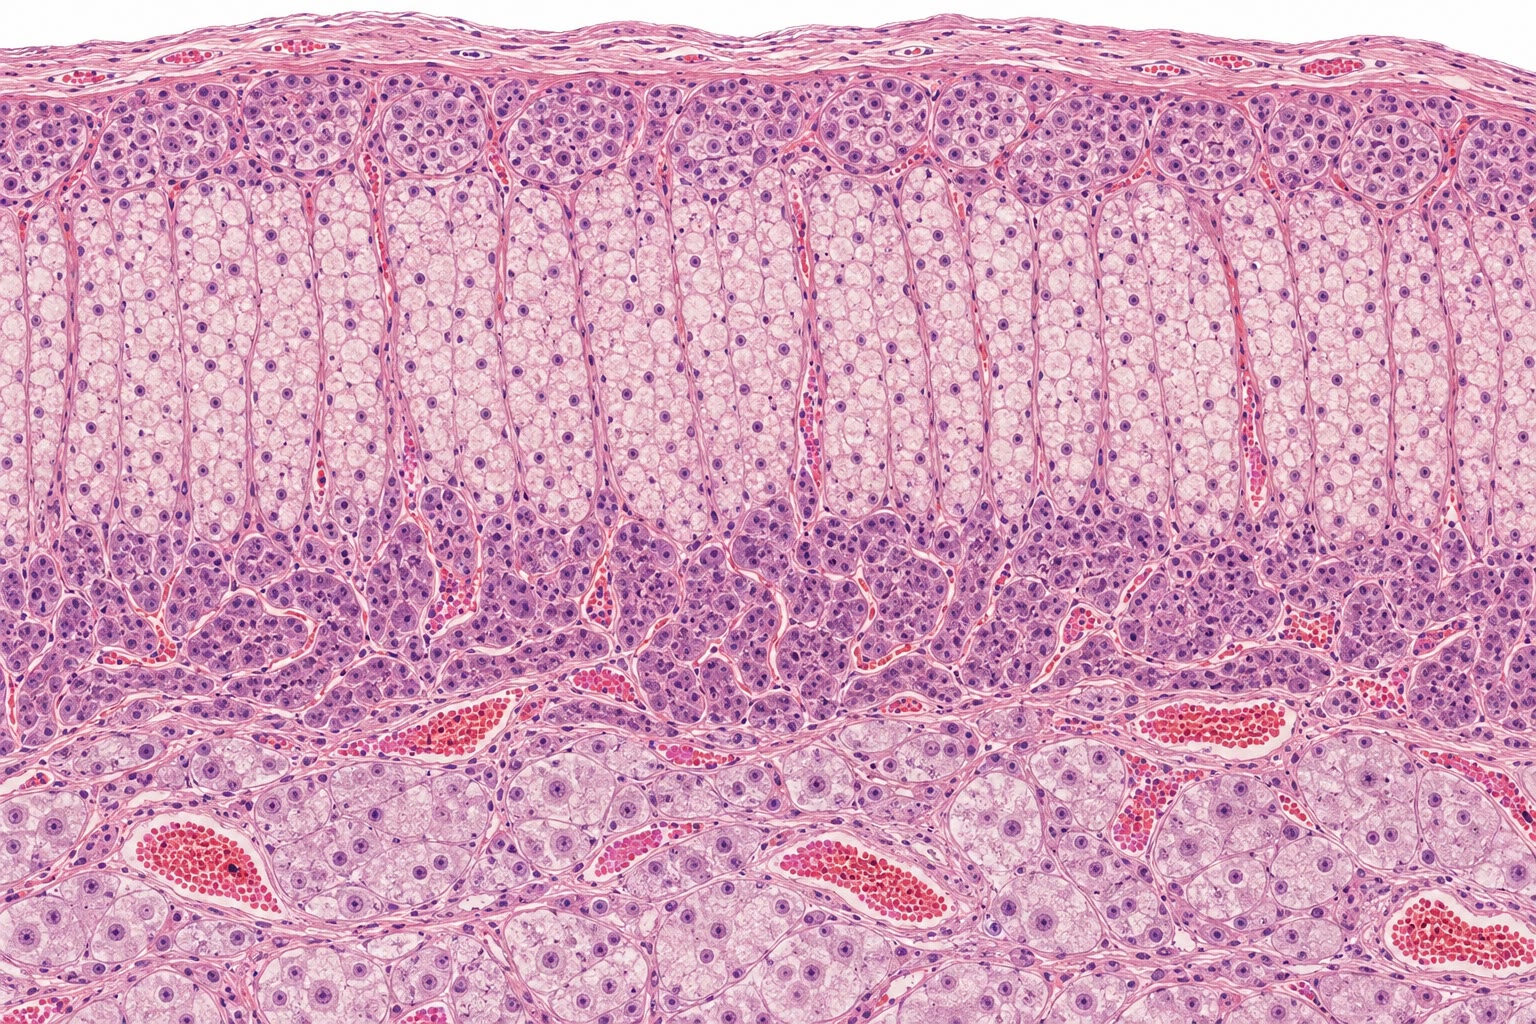
\includegraphics[width=0.5\linewidth]{images/book5/ai/b5-21-adrenal-section.jpg}\hspace{0.04\linewidth}
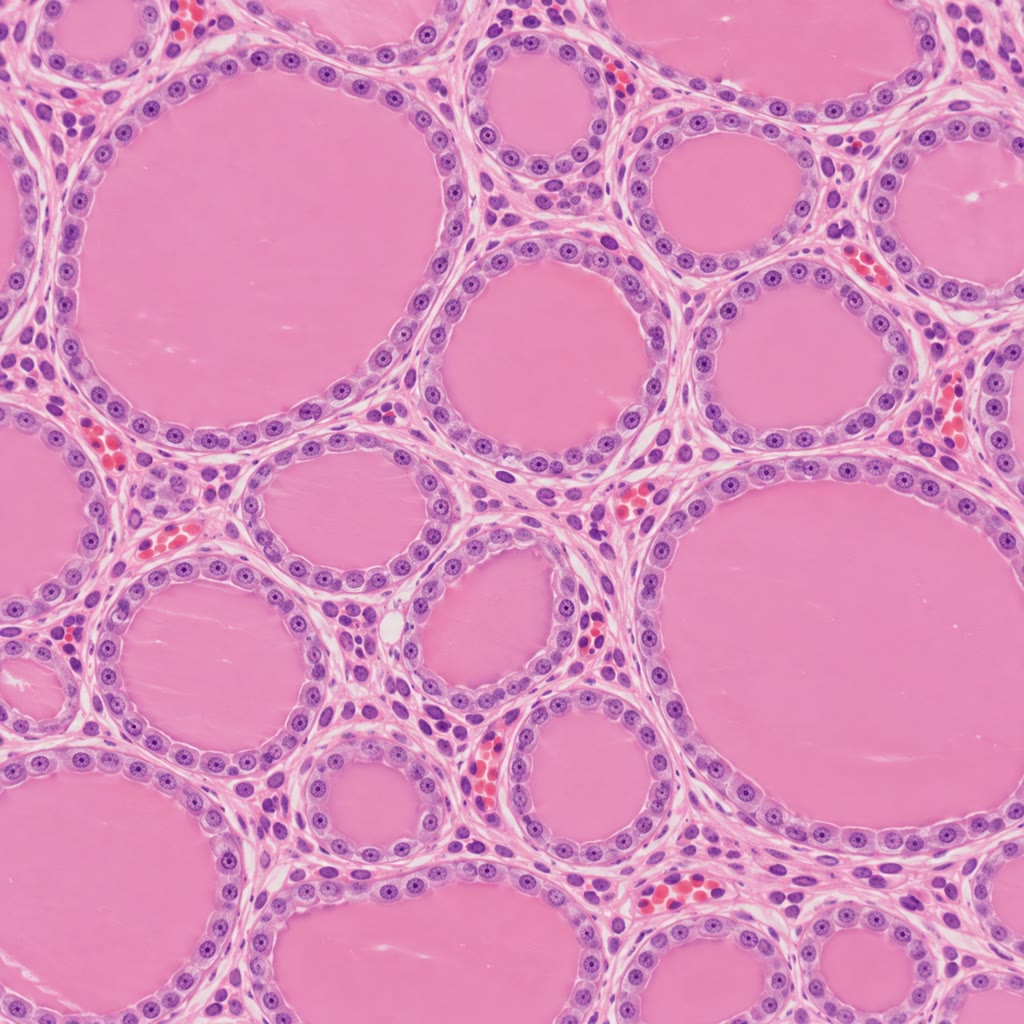
\includegraphics[width=0.36\linewidth]{images/book5/ai/b5-21-thyroid-follicles.jpg}

{\small 左：肾上腺切面——皮质分为三个区
（外层为\omterm{def:b3:renal-osmoregulation:controls}{醛固酮}，宽阔的中间带为皮质醇，
最内层为雄\omterm{def:b3:endocrinology:hormone}{激素}），环绕着分泌肾上腺素的
嗜铬细胞构成的髓质，髓质就起源而言属于交感\omterm{def:b3:nervous-systems:comparative}{神经节}。右：
甲状腺滤泡，每个滤泡是围绕胶体储存库的细胞球，
胶体中以甲状腺球蛋白结合着可供数月使用的\omterm{def:b3:endocrinology:hormone}{激素}。}
\end{omfigure}

\section{葡萄糖：最紧的回路}

\begin{definition}[胰岛素与胰高血糖素]\label{def:b3:endocrinology:glucose}
\index{胰岛素}\index{胰高血糖素}\index{朗格汉斯岛}\index{GLUT4}\index{糖尿病}
血液中约含 \qty{5}{g} 葡萄糖，浓度为 \qty{5}{mmol/L}
（\qty{90}{mg/dL}），大脑每天消耗 \qty{120}{g}，且只能烧
葡萄糖，别无他物可烧；一餐可在一小时内提供 \qty{75}{g} 葡萄糖。
\emph{朗格汉斯岛}由约一百万个小团簇构成，每团含几千个细胞，
散布于胰腺中，掌控着这一回路。$\beta$ 细胞
通过代谢葡萄糖来感知其浓度：葡萄糖越多，ATP 越多，ATP 敏感的
钾通道关闭，细胞去极化，钙离子内流，并
促使\emph{胰岛素}胞吐释放，它是由单一前体切割而成的
\omterm{def:b3:endocrinology:hormone}{肽类激素}。胰岛素促使肌肉和脂肪将转运蛋白
\emph{GLUT4}\omterm{def:b3:cancer-biology:hallmarks}{转移}至细胞表面并摄取葡萄糖，促使肝脏将葡萄糖
以糖原形式储存并停止生成葡萄糖，促使脂肪停止释放脂肪
酸：它是进食状态下的\omterm{def:b3:endocrinology:hormone}{激素}，是唯一能降低
血糖的\omterm{def:b3:endocrinology:hormone}{激素}。$\alpha$ 细胞
在血糖下降时释放\emph{胰高血糖素}：肝脏分解糖原，并从氨基
酸与乳酸合成新的葡萄糖。肾上腺素、皮质醇和生长\omterm{def:b3:endocrinology:hormone}{激素}同样升高血糖，
而这种冗余并不对称：机体可以通过四条途径
抵御血糖下降，却只能通过一条途径应对血糖升高。\emph{糖尿
病}是这一条途径失效的结果：1 型是\omterm{def:b3:adaptive-immunity:tolerance}{自身免疫}
性破坏 $\beta$ 细胞，从第一天起就需要胰岛素；
2 型占十分之九，始于组织对
胰岛素产生抵抗，多年间靠更多的胰岛素代偿，直至 $\beta$ 细胞
无法跟上，血糖随之升高。
\end{definition}

\begin{theorem}[胰岛素–葡萄糖回路]\label{thm:b3:endocrinology:loop}
\index{环路增益}\index{调定点}\index{阻尼振荡}
设 $g$ 和 $i$ 分别为血浆葡萄糖和\omterm{def:b3:endocrinology:glucose}{胰岛素}
相对于空腹值的偏差。葡萄糖的清除速率与其自身的
过量（葡萄糖效能 $a$）成正比，并与\omterm{def:b3:endocrinology:glucose}{胰岛素}的过量
（敏感性 $s$）成正比；\omterm{def:b3:endocrinology:glucose}{胰岛素}的分泌与葡萄糖
的过量（$\beta$）成正比，并以速率 $\gamma$ 被清除；负荷 $u$ 进入系统：
\[
\dot g = -a\,g - s\,i + u, \qquad \dot i = \beta\,g - \gamma\,i .
\]
在恒定负荷 $u$ 下，葡萄糖稳定在
\[
g^{*} = \frac{u}{a}\cdot\frac{1}{1 + L}, \qquad L = \frac{s\beta}{a\gamma},
\]
因此，反馈将无调节机体所承受的扰动
降为原来的 $1 + L$ 分之一，此因子即\emph{\omterm{thm:b3:endocrinology:loop}{环路增益}}加一。一次大剂量注入后
恢复过程由本征值决定：
$\lambda = -\tfrac{a + \gamma}{2} \pm \sqrt{\tfrac{(a+\gamma)^{2}}{4} - (a\gamma + s\beta)}$：
若 $s\beta < (a - \gamma)^{2}/4$，则单调恢复；否则为\omterm{thm:b3:endocrinology:loop}{阻尼
振荡}，角频率 $\omega = \sqrt{a\gamma + s\beta -
(a+\gamma)^{2}/4}$ 按 $\mathrm{e}^{-(a+\gamma)t/2}$ 衰减——血糖
在稳定之前会略低于其空腹值，此即甜食后两三小时出现的
轻度低血糖。\omterm{def:b3:endocrinology:glucose}{胰岛素}
抵抗会降低 $s$：在机体自身肝脏输出的作用下，空腹稳态时
血糖升高，回路以更高的 $i^{*}$ 代偿，
直至 $\beta$ 细胞的 $\beta$ 也下降，代偿随之失效。
\end{theorem}
\begin{proof}
稳态：由 $\dot i = 0$ 得 $i^{*} = \beta g^{*}/\gamma$；
代入 $\dot g = 0$：$a g^{*} + s\beta g^{*}/\gamma = u$，于是 $g^{*} =
u/(a + s\beta/\gamma) = (u/a)/(1 + L)$。动力学：系统矩阵为
$\begin{pmatrix} -a & -s\\ \beta & -\gamma\end{pmatrix}$，迹为
$-(a+\gamma)$，行列式为 $a\gamma + s\beta$；其特征
方程 $\lambda^{2} + (a+\gamma)\lambda + (a\gamma + s\beta) = 0$ 的根
即上文所述。两根的实部均为负，故空腹状态
稳定；当判别式 $(a+\gamma)^{2}
- 4(a\gamma + s\beta) = (a-\gamma)^{2} - 4s\beta$ 为负时根为复数，
即所给条件，此时 $g(t) = \mathrm{e}^{-(a+\gamma)t/2}(A\cos\omega t
+ B\sin\omega t)$，并穿过零点。抵抗：当 $u$ 为肝脏的
基础输出且 $s$ 降低时，$L$ 下降，$g^{*}$ 升高，对相同的
$u$；$i^{*} = \beta g^{*}/\gamma$ 随之升高（高\omterm{def:b3:endocrinology:glucose}{胰岛素}血症）；
若 $\beta$ 随后下降，$L$ 进一步下降，$g^{*}$ 则趋向 $u/a$。
\end{proof}

\begin{omfigure}
\begin{tikzpicture}
\begin{axis}[
  width=0.58\linewidth, height=5.6cm,
  axis x line=bottom, axis y line=left,
  xmin=0, xmax=180, ymin=40, ymax=200,
  xlabel={葡萄糖负荷后的分钟数}, ylabel={血浆葡萄糖 (mg/dL)},
  xlabel style={font=\small, at={(axis description cs:0.5,-0.12)}, anchor=north}, ylabel style={font=\small},
  tick label style={font=\small}, xtick={0,30,60,90,120,150,180}, ytick={60,90,120,150,180},
  clip=false,
]
\addplot[very thick, omDef, smooth] coordinates {(0,190) (6,165) (12,131) (18,102) (24,84) (30,77) (36,78) (42,82) (48,86) (54,89) (60,91) (66,92) (72,91) (78,91) (84,90) (90,90) (96,90) (102,90) (108,90) (114,90) (120,90) (126,90) (132,90) (138,90) (144,90) (150,90) (156,90) (162,90) (168,90) (174,90) (180,90)};
\draw[dashed, gray] (axis cs:0,90) -- (axis cs:180,90);
\node[font=\scriptsize, gray, anchor=south east] at (axis cs:180,91) {空腹水平};
\node[font=\scriptsize, omDef, anchor=west, align=left] at (axis cs:75,150) {模型：$a = \qty{0.02}{min^{-1}}$，$\gamma = \qty{0.1}{min^{-1}}$，\\$s\beta = \qty{0.01}{min^{-2}}$，环路增益 $L = 5$；\\下冲出现于 \qty{32}{min}，周期 \qty{68}{min}};
\node[font=\scriptsize, omThm, anchor=north] at (axis cs:24,70) {下冲};
\end{axis}
\begin{axis}[
  at={(0.6\linewidth,0)}, anchor=south west,
  width=0.33\linewidth, height=5.6cm,
  axis x line=bottom, axis y line=left,
  xmin=0, xmax=180, ymin=0, ymax=40,
  xlabel={分钟}, ylabel={胰岛素 (mU/L)},
  xlabel style={font=\small, at={(axis description cs:0.5,-0.12)}, anchor=north}, ylabel style={font=\small},
  tick label style={font=\small}, xtick={0,60,120,180}, ytick={0,10,20,30,40},
]
\addplot[very thick, omProp, smooth] coordinates {(0,10.0) (6,30.0) (12,33.7) (18,28.5) (24,20.4) (30,13.4) (36,8.9) (42,7.1) (48,7.1) (54,7.9) (60,9.0) (66,9.8) (72,10.2) (78,10.4) (84,10.4) (90,10.2) (96,10.1) (102,10.0) (108,10.0) (114,9.9) (120,10.0) (126,10.0) (132,10.0) (138,10.0) (144,10.0) (150,10.0) (156,10.0) (162,10.0) (168,10.0) (174,10.0) (180,10.0)};
\draw[dashed, gray] (axis cs:0,10) -- (axis cs:180,10);
\end{axis}
\end{tikzpicture}

{\small 葡萄糖负荷后的线性环路，该负荷使血糖升高
\qty{100}{mg/dL}。\omterm{def:b3:endocrinology:glucose}{胰岛素}在十分钟内达到峰值，二十分钟内血糖
回到基线，随后出现下冲；一种经由自身清除时间较长的\omterm{def:b3:endocrinology:hormone}{激素}起作用的强反馈，
使其以\omterm{thm:b3:endocrinology:loop}{阻尼振荡}的形式回落，
而非简单衰减。}
\end{omfigure}

\begin{proof}[证据]
冯·梅林与闵可夫斯基（1889 年）切除了一只狗的胰腺，使其患上\omterm{def:b3:endocrinology:glucose}{糖尿病}——
围聚在其尿液上的苍蝇泄露了糖分的秘密；结扎
导管则不然，此法破坏了消化组织，却保住了胰岛，
因而未引发\omterm{def:b3:endocrinology:glucose}{糖尿病}。班廷与贝斯特（1921 年）在柯利普的协助下提纯，
提取出\omterm{def:b3:endocrinology:glucose}{胰岛素}，使一只\omterm{def:b3:endocrinology:glucose}{糖尿病}狗的血糖降低，随后用于
莱纳德·汤普森（1922 年 1 月）的治疗。桑格测定了\omterm{def:b3:endocrinology:glucose}{胰岛素}的序列（1955 年），
它是首个被测定序列的蛋白质；雅洛与伯森在血液中测定了它
（1959 年），发现成年发病的\omterm{def:b3:endocrinology:glucose}{糖尿病}患者起初体内的\omterm{def:b3:endocrinology:glucose}{胰岛素}反而比健康人多——
这说明的是抗性，而非缺乏。基因泰克公司的细菌于 1978 年
制成了人\omterm{def:b3:endocrinology:glucose}{胰岛素}，这是第一种重组药物。
\end{proof}

\begin{omfigure}
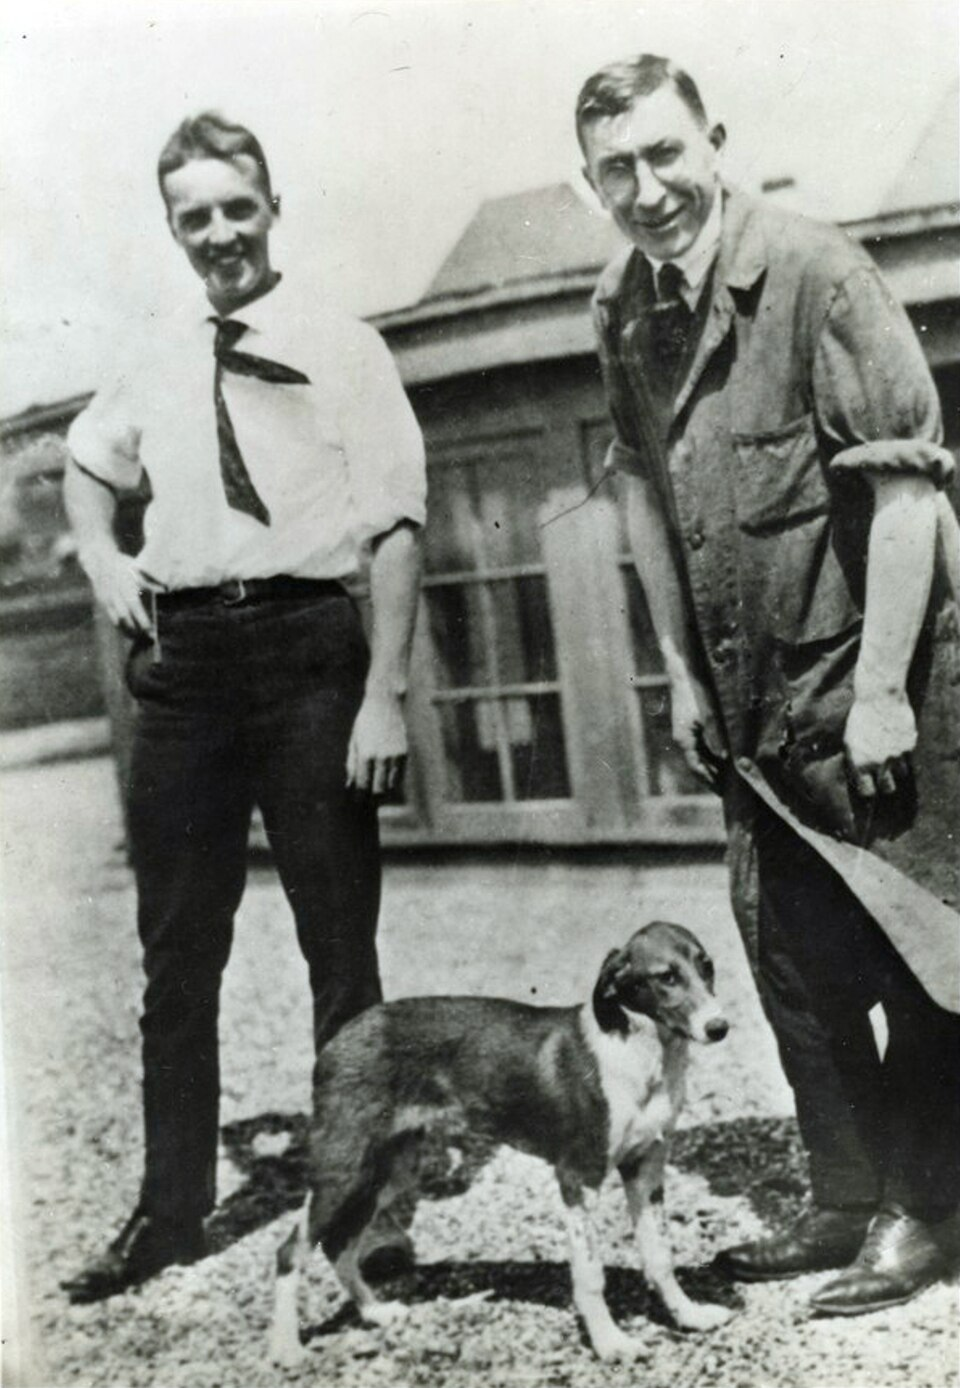
\includegraphics[width=0.42\linewidth]{images/book5/banting-best.jpg}\hspace{0.04\linewidth}
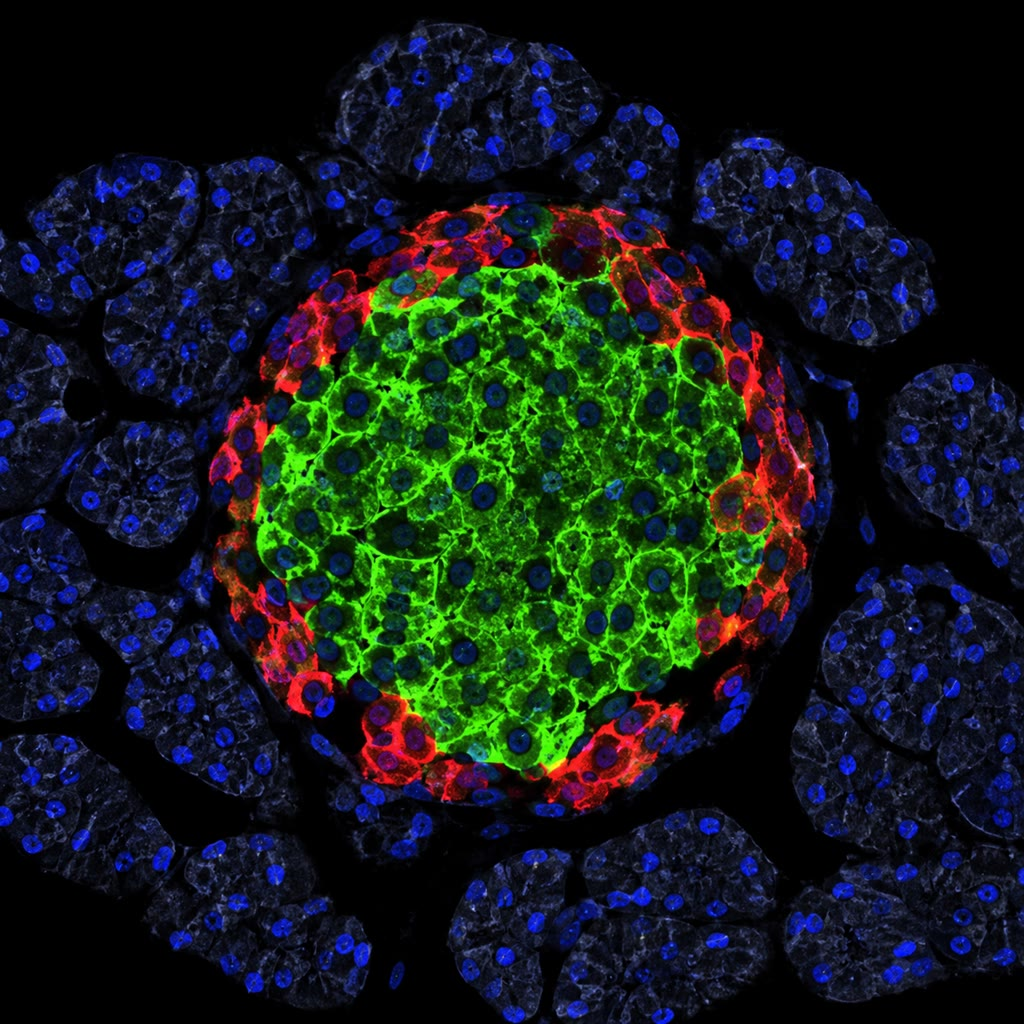
\includegraphics[width=0.42\linewidth]{images/book5/ai/b5-21-pancreatic-islet.jpg}

{\small 左：弗雷德里克·班廷与查尔斯·贝斯特在
多伦多医学楼楼顶，约摄于 1924 年，身旁是\omterm{def:b3:endocrinology:glucose}{胰岛素}实验中的一只狗（照片属公有领域）。右图：
一个\omterm{def:b3:endocrinology:glucose}{朗格汉斯岛}，中心为产生\omterm{def:b3:endocrinology:glucose}{胰岛素}的 $\beta$ 细胞，
边缘为分泌\omterm{def:b3:endocrinology:glucose}{胰高血糖素}的 $\alpha$ 细胞，
浸没在外分泌腺泡之中。}
\end{omfigure}

\begin{method}[读取患者的血糖环路]\label{met:b3:endocrinology:ogtt}
\index{葡萄糖耐量试验}\index{HbA1c}
(1) 空腹血浆葡萄糖：低于 \qty{5.6}{mmol/L} 为正常，
两次测定值均在 \qty{7.0}{mmol/L} 或以上即为\omterm{def:b3:endocrinology:glucose}{糖尿病}。(2) 口服\omterm{met:b3:endocrinology:ogtt}{葡萄糖耐量试验}：
服用 \qty{75}{g} 葡萄糖，两小时血浆葡萄糖低于
\qty{7.8}{mmol/L} 为正常，达到或超过 \qty{11.1}{mmol/L} 即为\omterm{def:b3:endocrinology:glucose}{糖尿病}——
两小时值反映环路的增益，空腹值反映其\omterm{thm:b3:endocrinology:loop}{调定
点}。(3) 糖化血红蛋白 \emph{\omterm{met:b3:endocrinology:ogtt}{HbA1c}}：葡萄糖与血红蛋白
不可逆地结合，速率正比于其浓度；红细胞寿命为 120 天，因此糖化比例
综合了过去三个月的平均血糖，且无需禁食。
正常值低于 \qty{5.7}{\%}，\omterm{def:b3:endocrinology:glucose}{糖尿病}则为 \qty{6.5}{\%} 及以上。
(4) 要将抗性与缺乏区分开，应同时测定
\omterm{def:b3:endocrinology:glucose}{胰岛素}（或其副产物 C 肽）：\omterm{def:b3:endocrinology:glucose}{胰岛素}与血糖均高，
即为抗性；
C 肽缺失，则为 1 型。
\end{method}

\section{钙与生物钟}

\begin{definition}[钙稳态]\label{def:b3:endocrinology:calcium}
\index{甲状旁腺激素}\index{骨化三醇}\index{维生素 D}\index{骨质疏松症}
血浆中的离子钙被稳定在 \qty{1.2}{mmol/L}，波动仅在百分之几之内，
因为它决定着每一条神经和肌肉的兴奋性：钙过低时，
它们会自发放电（手足搐搦），钙过高时则
变得迟钝。四个甲状旁腺借助表面受体感知钙浓度，
并沿陡峭的反 S 形曲线分泌\emph{甲状旁腺\omterm{def:b3:endocrinology:hormone}{激素}}（PTH）：
PTH 促使骨中的钙动员入血，并使肾脏重吸收钙，
使肾脏排出磷酸盐，又激活\emph{维生素 D}——它可在皮肤中经紫外线照射生成，
或经食物摄入，先在肝脏羟基化，再在肾脏中转化为
\emph{骨化三醇}——它促使肠道吸收钙。骨骼
是钙的储库，约含一千克钙，
在甲状旁腺\omterm{def:b3:endocrinology:hormone}{激素}、骨化三醇、雌\omterm{def:b3:endocrinology:hormone}{激素}与负荷的作用下，由破骨细胞与成骨细胞持续重塑。
维生素 D 缺乏，儿童会患佝偻病，成人则骨质软化；
绝经时雌\omterm{def:b3:endocrinology:hormone}{激素}下降，使重塑偏向骨吸收，
并导致\emph{骨质疏松症}；甲状旁腺腺瘤会使血钙升高，
使骨质溶解并形成肾结石——“骨头、结石、
呻吟与抱怨。”
\end{definition}

\begin{definition}[昼夜节律钟]\label{def:b3:endocrinology:clock}
\index{昼夜节律钟}\index{视交叉上核}\index{时钟基因}\index{褪黑素}\index{授时因子}
几乎每个细胞都带有一个\emph{昼夜节律钟}：它是一个
转录–翻译环路，其中 CLOCK 与 BMAL1 两种蛋白质
激活基因 \emph{Per} 与 \emph{Cry}，其蛋白质
逐渐积累，经数小时的延迟后进入细胞核，并抑制自身的转录，
随后被降解，解除抑制——一个
循环约为二十四小时，由延迟与降解的速率
所决定。人体各处的生物钟由一个主时钟同步，
该主时钟由两万个神经元组成，位于\omterm{def:b3:endocrinology:axes}{下丘脑}的\emph{视交叉上核}中，
而它本身又受光线调节，光线经由一类专门的
\omterm{def:b3:sensory-systems:retina}{视网膜}\omterm{def:b3:sensory-systems:retina}{神经节细胞}（含黑视蛋白，而非\omterm{def:b3:sensory-systems:retina}{视杆细胞}或
\omterm{def:b3:sensory-systems:retina}{视锥细胞}的色素）传入，并通过松果体的
\emph{褪黑素}向全身发出黑夜信号，该\omterm{def:b3:endocrinology:hormone}{激素}仅在黑暗中分泌。时钟
安排皮质醇在醒前分泌，体温在凌晨 4 点最低，
生长\omterm{def:b3:endocrinology:hormone}{激素}在入睡后的第一段睡眠中分泌，\omterm{def:b3:endocrinology:glucose}{胰岛素}敏感性在
早晨较高。食物、运动与温度是次要的
\emph{授时因子}，它们能把外周生物钟拉离
中央生物钟，这正是轮班工作者与时差反应之苦的根源——
肝脏的生物钟走的是一套时间，大脑则走另一套。
\end{definition}

\begin{proof}[证据]
科诺普卡与本泽尔（1971）筛选了羽化节律发生改变的突变果蝇，
发现同一基因 \emph{period} 有三个等位基因：短日型
（19 小时）、长日型（29 小时）及完全无节律型——一个带有
遗传周期的时钟。哈丁、霍尔与罗斯巴什（1990）发现，
\emph{period} 的 mRNA 与蛋白质均呈振荡，二者之间存在滞后，并且
该蛋白抑制其自身基因：即这一环路。拉尔夫与梅纳克
（1990）将一只具有
20 小时节律的突变仓鼠的\omterm{def:b3:endocrinology:clock}{视交叉上核}移植到一只自身\omterm{def:b3:endocrinology:clock}{视交叉上核}
已被毁坏的正常仓鼠体内：受体动物随之以 20 小时运行——这一周期
属于被移植的组织。被置于无时间线索的地下掩体中的人类，其
节律以略超过 24 小时的周期自由运行；傍晚的强光
使之延迟，清晨的强光则使之提前。
\end{proof}

\begin{omfigure}
\begin{tikzpicture}[every node/.style={font=\scriptsize}, >=stealth]
  \node[draw, thick, rounded corners, fill=omDef!20, align=center] (cb) at (0,1.6) {CLOCK--BMAL1\\激活剂};
  \node[draw, thick, rounded corners, fill=omProp!25, align=center] (pc) at (3.6,1.6) {\emph{Per}, \emph{Cry}\\被转录};
  \node[draw, thick, rounded corners, fill=omThm!20, align=center] (pr) at (3.6,-0.4) {PER、CRY 蛋白 \\积累、二聚化};
  \node[draw, thick, rounded corners, fill=omMeth!25, align=center] (nu) at (0,-0.4) {数小时后 \\进入细胞核};
  \draw[->, thick] (cb) -- (pc) node[midway, above, font=\tiny] {激活};
  \draw[->, thick] (pc) -- (pr) node[midway, right, font=\tiny] {翻译，延迟};
  \draw[->, thick] (pr) -- (nu);
  \draw[-|, thick, omThm] (nu) -- (cb) node[midway, left, font=\tiny, omThm, align=right] {抑制 \\自身的 \\激活剂};
  \draw[->, thick, gray] (nu.south) -- ++(0,-0.5) node[below, font=\tiny, gray] {降解：抑制解除，循环重新开始 $\approx$ \qty{24}{h}};
  % right: daily profile
  \begin{scope}[shift={(7.2,-1.6)}]
    \draw[->] (0,0) -- (5.6,0) node[right, font=\tiny] {小时};
    \draw[->] (0,0) -- (0,3.4);
    \foreach \x/\l in {0/0, 1.4/6, 2.8/12, 4.2/18, 5.6/24} { \draw (\x,0) -- (\x,-0.08) node[below, font=\tiny] {\l}; }
    \fill[gray!25] (0,0) rectangle (1.4,3.4); \fill[gray!25] (5.1,0) rectangle (5.6,3.4);
    \node[font=\tiny, gray!60!black] at (0.7,3.2) {夜晚};
    \draw[very thick, omMeth!70!black, domain=0:5.6, samples=60, smooth, variable=\x] plot (\x, {1.6 + 1.2*cos(deg(2*3.1416*(\x-1.9)/5.6))});
    \node[font=\tiny, omMeth!70!black] at (3.1,3.1) {皮质醇：上午 8 点达峰值};
    \draw[very thick, omDef, domain=0:5.6, samples=60, smooth, variable=\x] plot (\x, {0.9 + 0.7*cos(deg(2*3.1416*(\x-0.7)/5.6))});
    \node[font=\tiny, omDef] at (2.7,0.18) {褪黑素：仅夜晚分泌};
  \end{scope}
\end{tikzpicture}

{\small 左：分子钟的核心，一个具有数小时延迟的\omterm{def:b3:endocrinology:axes}{负反馈}环路，
这正是环路振荡而非趋于稳定所需要的。
右：该时钟所调度的两种\omterm{def:b3:endocrinology:hormone}{激素}——皮质醇在
黎明前升高，为新的一天做准备；\omterm{def:b3:endocrinology:clock}{褪黑素}则标志着夜晚。}
\end{omfigure}

\begin{remark}[作为控制的稳态]\label{rem:b3:endocrinology:control}
本章中的每个环路都具有相同的组成部分：感受器（$\beta$ 细胞的代谢、
甲状旁腺的钙受体、\omterm{def:b3:endocrinology:axes}{垂体}的\omterm{prop:b3:endocrinology:thyroid}{甲状腺激素}受体）、将信号与\omterm{thm:b3:endocrinology:loop}{调定点}相比较的控制器、
带有自身半衰期的效应\omterm{def:b3:endocrinology:hormone}{激素}，以及一种反馈：
使误差减小为 $1 + L$ 分之一，
但永远不会减为零。
各环路的不同之处在于时间尺度——肾上腺素以秒计，
\omterm{def:b3:endocrinology:glucose}{胰岛素}以小时计，甲状腺素以天计，骨则以一生计 ---
以及这种折中的代价：反应快而效应滞后的环路会发生振荡，缓慢的环路
则会使扰动持续存在。临床医生从外部观察这些环路，
即通过反馈所耦合的成对指标：TSH 高而 T$_{4}$ 低，
说明是腺体衰竭；TSH 高而 T$_{4}$ 也高，则说明是\omterm{def:b3:endocrinology:axes}{垂体}衰竭；
\omterm{def:b3:endocrinology:glucose}{胰岛素}高而血糖高，属\omterm{def:b3:endocrinology:glucose}{胰岛素}抵抗；
\omterm{def:b3:endocrinology:glucose}{胰岛素}低而血糖高，是破坏。读取某种\omterm{def:b3:endocrinology:hormone}{激素}的水平时，
必须始终追问其指挥者当时在做什么。
\end{remark}

\section{练习}

\begin{exercise}[$\star$]\label{exo:b3:endocrinology:1}
对\omterm{def:b3:endocrinology:glucose}{胰岛素}、皮质醇、肾上腺素、甲状腺素和加压素，
按化学性质、受体位置、作用速度及半衰期进行分类。
\end{exercise}

\begin{exercise}[$\star$]\label{exo:b3:endocrinology:2}
画出甲状腺轴及其反馈，并预测以下情况下 TSH 与 T$_{4}$ 的水平：
甲状腺被破坏；分泌 TSH 的\omterm{def:b3:endocrinology:axes}{垂体}\omterm{def:b3:cancer-biology:hallmarks}{肿瘤}；患者
服用过量甲状腺素；碘缺乏。
\end{exercise}

\begin{exercise}[$\star$]\label{exo:b3:endocrinology:3}
为什么机体有四种能升高血糖的\omterm{def:b3:endocrinology:hormone}{激素}，
而能降低血糖的\omterm{def:b3:endocrinology:hormone}{激素}却只有一种？这一点对\omterm{def:b3:endocrinology:glucose}{胰岛素}过多与过少的相对危害
有何预测？
\end{exercise}

\begin{exercise}[$\star$]\label{exo:b3:endocrinology:4}
什么是\omterm{def:b3:endocrinology:clock}{授时因子}？举出三种，说明主时钟使用哪一种，
并解释跨越八个时区的旅行者会出现什么情况。
\end{exercise}

\begin{exercise}[$\star\star$]\label{exo:b3:endocrinology:5}
某细胞有 \num{20000} 个受体，其 $K_{d} = \qty{1}{nM}$，且
\num{500} 个受体被占据时反应达到最大。求 EC$_{50}$。经过一周的高\omterm{def:b3:endocrinology:hormone}{激素}作用后，
该细胞有 \num{2000} 个受体：新的 EC$_{50}$ 是多少？
请就\omterm{def:b3:endocrinology:glucose}{胰岛素}抵抗加以解释。
\end{exercise}

\begin{exercise}[$\star\star$]\label{exo:b3:endocrinology:6}
取 $\kappa = \qty{0.46}{L/pmol}$，正常 TSH 为 \qty{1.5}{mU/L}，
游离 T$_{4}$ 为 \qty{15}{pmol/L} 时，计算游离 T$_{4}$ 为 $13$、
$11$、$9$ 和 \qty{25}{pmol/L} 时的 TSH。在上述哪些取值下，T$_{4}$ 仍
处于 \qtyrange{10}{20}{pmol/L} 的参考范围内，而 TSH
却超出 \qtyrange{0.4}{4}{mU/L}？
\end{exercise}

\begin{exercise}[$\star\star$]\label{exo:b3:endocrinology:7}
对于\cref{thm:b3:endocrinology:loop}中的环路，取 $a = \qty{0.02}{min^{-1}}$，
$\gamma = \qty{0.1}{min^{-1}}$, $\beta = \qty{0.05}{mU\,L^{-1}\,min^{-1}}$
（每 mg/dL）、$s = \qty{0.2}{mg\,dL^{-1}\,min^{-1}}$（每 mU/L），
计算\omterm{thm:b3:endocrinology:loop}{环路增益}、在恒定负荷
\qty{2}{mg/dL/min} 下的稳态血糖过量、无反馈时的同一数值，以及稳态\omterm{def:b3:endocrinology:glucose}{胰岛素}
过量。
\end{exercise}

\begin{exercise}[$\star\star$]\label{exo:b3:endocrinology:8}
参数同上：经过一次推注后，回落是否为振荡的？计算
周期，以及振幅降至原来的 $\mathrm{e}$ 分之一所需的时间。现将
$s$ 减半（\omterm{def:b3:endocrinology:glucose}{胰岛素}抵抗），重新计算这两个量以及新的\omterm{thm:b3:endocrinology:loop}{环路增益}。
\end{exercise}

\begin{exercise}[$\star\star$]\label{exo:b3:endocrinology:9}
皮质醇的半衰期为 \qty{80}{min}。一名患者每天服用 \qty{40}{mg} 的
泼尼松龙，持续一年后突然停药。逐级解释，
为何该患者可能在三天后因轻微感染而崩溃，并
说明若测量该轴，结果会显示什么（ACTH、皮质醇、对
注射 ACTH 的反应）。
\end{exercise}

\begin{exercise}[$\star\star\star$]\label{exo:b3:endocrinology:10}
证明：对单变量\omterm{def:b3:endocrinology:axes}{负反馈} $\dot x = f(x)$，若 $f' < 0$，
则其不能振荡，而定理中的双变量环路可以振荡，并
用文字解释，为何生物钟需要在转录与抑制之间存在数小时的延迟，
才能产生 24 小时的周期。若 PER 的降解速度加快一倍，
周期会如何变化？
\end{exercise}

\begin{exercise}[$\star\star\star$]\label{exo:b3:endocrinology:11}
\omterm{def:b3:endocrinology:calcium}{甲状旁腺激素}满足 $\text{PTH} = P_{\max}/(1 +
\mathrm{e}^{k(\text{Ca} - \text{Ca}_{0})})$，其中 $\text{Ca}_{0} =
\qty{1.2}{mmol/L}$，$k = \qty{20}{L/mmol}$。计算 PTH
占最大值的比例，在 Ca $= 1.10$、$1.15$、$1.20$、$1.25$ 和 \qty{1.30}{mmol/L} 时
求\omterm{thm:b3:endocrinology:loop}{调定点}处的斜率，并解释为何钙需要如此陡峭的响应，
而血糖若如此则会有危险。
\end{exercise}

\begin{exercise}[$\star\star\star$]\label{exo:b3:endocrinology:12}
葡萄糖以每单位时间 $k\,G$ 的速率与血红蛋白结合，其中
$k$ 的取值使平均葡萄糖浓度为 \qty{5.5}{mmol/L} 时糖化比例达到 \qty{5}{\%}，
即红细胞 120 天寿命内的糖化。推导 \omterm{met:b3:endocrinology:ogtt}{HbA1c} 作为
平均葡萄糖浓度的函数，求其在 \qty{10}{mmol/L} 时的值，并解释为何一名
患有溶血性贫血（红细胞寿命为 60 天）的患者，其 \omterm{met:b3:endocrinology:ogtt}{HbA1c} 会
显得偏低，具有误导性。
\end{exercise}

\section{问题：血液中的糖}

\begin{problem}[{周末问题——通过线性\omterm{def:b3:endocrinology:glucose}{胰岛素}–葡萄糖环路解读\omterm{met:b3:endocrinology:ogtt}{葡萄糖耐量试验}：
\qty{75}{g} 剂量的分布，\omterm{thm:b3:endocrinology:loop}{环路增益}与阻尼回落，
\omterm{def:b3:endocrinology:glucose}{胰岛素}抵抗与 $\beta$ 细胞功能衰竭对空腹\omterm{thm:b3:endocrinology:loop}{调定点}的影响，
依据数值作出诊断，以及并列的甲状腺轴，
最后落在故障环路的\omterm{thm:b3:endocrinology:loop}{环路增益}、回落时间
与空腹血糖上}]
\label{pb:b3:endocrinology:1}
数据：健康成年人，葡萄糖分布容积 \qty{15}{L}，
空腹血糖 \qty{90}{mg/dL}（\qty{5}{mmol/L}），空腹\omterm{def:b3:endocrinology:glucose}{胰岛素}
\qty{10}{mU/L}。环路参数：$a = \qty{0.02}{min^{-1}}$，$\gamma =
\qty{0.1}{min^{-1}}$，$\beta = 0.05$（mU/L 每分钟每 mg/dL），$s = 0.2$
（mg/dL 每分钟每 mU/L）。基础肝糖输出 $u_{0} =
\qty{2}{mg/dL/min}$（空腹状态下已由
空腹清除量达到平衡）。口服 \qty{75}{g} 剂量在
一小时内吸收。甲状腺：$\text{TSH} = 1.5\,\mathrm{e}^{-0.46(T_{4} - 15)}$ mU/L。
葡萄糖摩尔质量 \qty{180}{g/mol}。

\medskip
\noindent\textbf{第一部分——剂量。}
\begin{enumerate}
  \item 将空腹血糖换算为 mmol/L，并核对
        由 mg/dL 换算而来。空腹时的
        分布容积中含有多少克葡萄糖？
  \item 若全部 \qty{75}{g} 一次性进入 \qty{15}{L}，血糖将升高多少
        （以 mg/dL 和 mmol/L 计）？为何实际
        峰值比空腹高约 \qty{60}{mg/dL}，远低于此？
  \item 若在 \qty{60}{min} 内吸收，剂量以何种速率
        （mg/dL 每分钟）进入？与 $u_{0}$ 比较。
  \item 若无任何\omterm{def:b3:endocrinology:glucose}{胰岛素}反应（$s = 0$），血糖将服从 $\dot
        g = -a g + u$。求在该吸收速率下的稳态过量，以及
        趋近过程的时间常数。一小时后
        血糖将处于何值？
  \item 计入环路，计算 $L$，以及在相同
        速率下的稳态过量。与第 4 题比较。
  \item 解释为何大脑在两方面都受到保护：它需要什么，
        以及过量葡萄糖多年来对组织造成什么影响。
\end{enumerate}

\medskip
\noindent\textbf{第二部分——回落。}
\begin{enumerate}[resume]
  \item 写出该环路的特征方程，并计算
        迹、行列式与判别式。
  \item 计算 $\omega$ 与\omterm{thm:b3:endocrinology:loop}{阻尼振荡}的周期，以及
        衰减时间 $2/(a + \gamma)$。
  \item 设初始过量为 \qty{100}{mg/dL}，\omterm{def:b3:endocrinology:glucose}{胰岛素}处于其
        空腹值，解为 $g(t) = 100\,\mathrm{e}^{-0.06t}
        (\cos\omega t + c\sin\omega t)$。求 $c$，由 $\dot g(0) = -a\cdot
        100$ 确定。
  \item 血糖何时首次回到空腹值（$g$ 的第一个零点）？
        估计第一个极小值处的过冲量。
  \item \omterm{def:b3:endocrinology:glucose}{胰岛素}：$i(t)$ 具有相同的指数因子与频率。由
        $\dot i = \beta g - \gamma i$ 论证，其峰值出现在
        血糖已开始下降之后、且在血糖降至空腹值之前。
  \item 为何实际耐量试验中吸收历时一小时
        而非推注，会在 30--60 分钟出现峰值，并在
        两小时内回落，而在三小时时仅有轻微低谷？
\end{enumerate}

\medskip
\noindent\textbf{第三部分——环路失效。}
\begin{enumerate}[resume]
  \item \omterm{def:b3:endocrinology:glucose}{胰岛素}抵抗使 $s$ 减半。新的 $L$ 为多少？肝脏的 $u_{0}$
        现由新的空腹稳态来平衡：以 $g^{*} = (u_{0}/a)/(1
        + L)$ 作为相对于理想化无调节基线的过量，求
        空腹血糖相对于健康
        状态升高多少（分别计算两个 $g^{*}$ 值再相减）。
  \item \omterm{def:b3:endocrinology:glucose}{胰岛素}抵抗状态下的空腹\omterm{def:b3:endocrinology:glucose}{胰岛素}：分别计算两种状态下的 $i^{*} = \beta
        g^{*}/\gamma$ 及其比值。临床上将此
        称为什么？
  \item 现在 $\beta$ 细胞衰竭：$\beta$ 同样降至原来的五分之一。
        新的 $L$ 与新的空腹过量为多少？换算为 mmol/L，并与
        \qty{7}{mmol/L} 的\omterm{def:b3:endocrinology:glucose}{糖尿病}诊断阈值比较。
  \item 在第 15 题的状态下，回落是否仍为振荡的？
        计算判别式，以及最慢
        模式的时间常数。
  \item 某患者空腹血糖为 \qty{8}{mmol/L}，空腹\omterm{def:b3:endocrinology:glucose}{胰岛素}
        为 \qty{30}{mU/L}，两小时值为 \qty{13}{mmol/L}。
        根据各组数据判断其类型与机制。
  \item 另一患者空腹血糖为 \qty{15}{mmol/L}，C 肽
        未能检出，并在两个月\omterm{def:b3:membrane-traffic:endocytosis}{内体}重下降 \qty{8}{kg}。作出诊断，并
        从组织在缺乏
        \omterm{def:b3:endocrinology:glucose}{胰岛素}时的表现解释体重下降。
  \item \omterm{met:b3:endocrinology:ogtt}{HbA1c}：若第一位患者的平均血糖为
        \qty{9}{mmol/L}，而 \qty{5.5}{mmol/L} 对应 \qty{5}{\%}，估计
        其 \omterm{met:b3:endocrinology:ogtt}{HbA1c}，假设二者成正比。
\end{enumerate}

\medskip
\noindent\textbf{第四部分——旁边的腺体。}
\begin{enumerate}[resume]
  \item 游离 T$_{4}$ 为 \qty{12}{pmol/L}。计算 TSH。T$_{4}$ 是否在
        \qtyrange{10}{20}{pmol/L} 范围内？TSH 是否在
        \qtyrange{0.4}{4}{mU/L} 范围内？此状态称为什么？
  \item T$_{4}$ 为 \qty{7}{pmol/L}：TSH 为多少？若患者 T$_{4}$ 为此值而
        TSH 为 \qty{0.3}{mU/L}，\omterm{def:b3:dna-repair:lesions}{损伤}位于何处？
  \item 甲状腺素的半衰期为 \qty{7}{d}。一名接受替代治疗的患者
        漏服一周药片。水平将下降至何种比例，
        为何漏服一周的危害小于漏服一天的
        皮质醇替代药物？
  \item 格雷夫斯病：\omterm{def:b3:adaptive-immunity:antibody}{抗体}占据 TSH 受体。预测
        T$_{4}$、TSH，以及对数线性关系对
        所测 TSH 的影响。
  \item 用一段文字解释，为何\omterm{def:b3:endocrinology:hormone}{激素}水平若脱离其上级\omterm{def:b3:endocrinology:hormone}{激素}的水平便毫无意义，
        并利用本章最后一条
        注中的四组数据加以说明。
  \item 总结：健康环路的\omterm{thm:b3:endocrinology:loop}{环路增益}（第 5 题）、回落的周期
        与衰减时间（第 8 题），以及
        故障环路的空腹血糖（第 15 题）。
\end{enumerate}
\end{problem}
